\section{Return-oriented programming in a nutshell}
\subsection{x86 crash course}
    \frame{
        \frametitle{Register set}
        \begin{description}
            \item[\eax] holds the return value of a function call.
            \item[\ebx] holds a pointer to some data.
            \item[\ecx] is used for counters in string- and loop instructions.
            \item[\edx] holds a I/O pointers.
            \item[\esi] is the source pointer in some instructions.
            \item[\edi] is the destination pointer in some instructions.
            \item[\ebp] is the stack frame- or base pointer.
            \item[\esp] is the stack pointer.
            \item[\eip] is the instruction pointer.
            \item[\efl] is the status and control register.
        \end{description}
    }

    \frame{
        \frametitle{Instruction set}
        \begin{tabular}{l|p{0.66\textwidth}}
            \mov\ \esp, \ebp    & Copies the stack pointer \esp\ to the base pointer \ebp.
            \\ \hline
            \push\ \ebp         & Updates the stack pointer \esp\ and writes the value of \ebp\ to the new top of the stack.
            \\ \hline
            \pop\ \ebp          & Reads the value at the top of the stack -- the memory location that \esp\ points to, writes it into \ebp\ and discards the value from the stack by adjusting \esp.
            \\ \hline
            \call\ func         & Pushes the return address, which is the address of the next instruction (\eip+5) onto the stack and jumps to the instruction labeled by "func:".
            \\ \hline
            \ret                & Pops the return address from the top of the stack and writes it into \eip.
        \end{tabular}
    }

    \frame{
        \frametitle{The stack}
        \begin{itemize}
            \item data section in a process' address space
            \item contains local variables and buffers
            \item arguments to function calls and return addresses are also implemented using the stack
            \item \xes-family of CPUs:
                  \begin{itemize}
                      \item stack grows from higher to lower memory addresses
                      \item memory is addressed byte-wise \\
                            \lto\ \push\ decrements \esp\ by 4,
                            \pop\ increments \esp\ by 4
                  \end{itemize}
        \end{itemize}
    }

    \frame{
        \frametitle{Function calls -- \cdecl}
        \begin{itemize}
            \item parameters are \push ed to the stack in reverse order
            \item \call\ pushes the address of the next instruction onto the stack
            \item function prologue (\enter):
                  \begin{itemize}
                      \item save the base pointer \ebp
                      \item copy \esp\ to \ebp\ for \bpa
                      \item decrement \esp\ to allocate stack memory for local variables
                  \end{itemize}
            \item function epilogue (\leave):
                  \begin{itemize}
                      \item discard local variables by copying \ebp\ to \esp
                      \item restore \ebp\ by popping it from the stack
                  \end{itemize}
            \item \ret\ pops the return address off the stack and jumps to it
        \end{itemize}
    }

    \frame{
        \frametitle{Function calls -- stack diagram}
        \begin{center}
            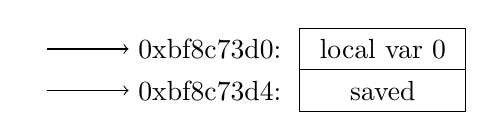
\begin{tikzpicture}
                \tikzset{x=2.5em, y=1.5em}
                \tikzstyle{mem}=[rectangle, draw, minimum width=6em, minimum height=1.5em]

                \draw (0.0, 1.0)    node        (esp)   {\esp};
                \draw (0.0, 0.0)    node        (ebp)   {\ebp};

                \draw (2.5, 1.0)    node        (a1)    {0xbf8c73d0:};
                \draw (2.5, 0.0)    node        (a0)    {0xbf8c73d4:};

                \draw (5.0, 1.0)    node[mem]   (s1)    {local var 0};
                \draw (5.0, 0.0)    node[mem]   (s0)    {saved \ebp};

                \draw [->]          (esp) -- (a1);
                \draw [->]          (ebp) -- (a0);
            \end{tikzpicture}
        \end{center}
    }

    \frame{
        \frametitle{Function calls -- stack diagram}
        \begin{center}
            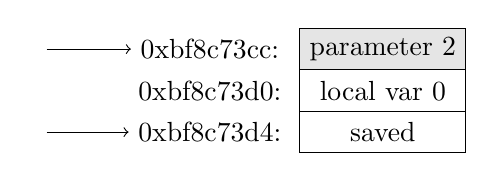
\begin{tikzpicture}
                \tikzset{x=2.5em, y=1.5em}
                \tikzstyle{mem}=[rectangle, draw, minimum width=6em, minimum height=1.5em]
                \tikzstyle{frame}=[mem, fill=black!10]

                \draw (0.0, 2.0)    node        (esp)   {\esp};
                \draw (0.0, 0.0)    node        (ebp)   {\ebp};

                \draw (2.5, 2.0)    node        (a2)    {0xbf8c73cc:};
                \draw (2.5, 1.0)    node        (a1)    {0xbf8c73d0:};
                \draw (2.5, 0.0)    node        (a0)    {0xbf8c73d4:};

                \draw (5.0, 2.0)    node[frame] (p2)    {parameter 2};
                \draw (5.0, 1.0)    node[mem]   (s1)    {local var 0};
                \draw (5.0, 0.0)    node[mem]   (s0)    {saved \ebp};

                \draw [->]          (esp) -- (a2);
                \draw [->]          (ebp) -- (a0);
            \end{tikzpicture}
        \end{center}
    }

    \frame{
        \frametitle{Function calls -- stack diagram}
        \begin{center}
            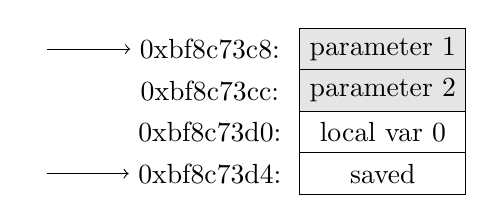
\begin{tikzpicture}
                \tikzset{x=2.5em, y=1.5em}
                \tikzstyle{mem}=[rectangle, draw, minimum width=6em, minimum height=1.5em]
                \tikzstyle{frame}=[mem, fill=black!10]

                \draw (0.0, 3.0)    node        (esp)   {\esp};
                \draw (0.0, 0.0)    node        (ebp)   {\ebp};

                \draw (2.5, 3.0)    node        (a3)    {0xbf8c73c8:};
                \draw (2.5, 2.0)    node        (a2)    {0xbf8c73cc:};
                \draw (2.5, 1.0)    node        (a1)    {0xbf8c73d0:};
                \draw (2.5, 0.0)    node        (a0)    {0xbf8c73d4:};

                \draw (5.0, 3.0)    node[frame] (p1)    {parameter 1};
                \draw (5.0, 2.0)    node[frame] (p2)    {parameter 2};
                \draw (5.0, 1.0)    node[mem]   (s1)    {local var 0};
                \draw (5.0, 0.0)    node[mem]   (s0)    {saved \ebp};

                \draw [->]          (esp) -- (a3);
                \draw [->]          (ebp) -- (a0);
            \end{tikzpicture}
        \end{center}
    }

    \frame{
        \frametitle{Function calls -- stack diagram}
        \begin{center}
            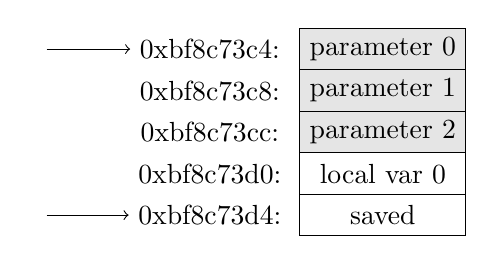
\begin{tikzpicture}
                \tikzset{x=2.5em, y=1.5em}
                \tikzstyle{mem}=[rectangle, draw, minimum width=6em, minimum height=1.5em]
                \tikzstyle{frame}=[mem, fill=black!10]

                \draw (0.0, 4.0)    node        (esp)   {\esp};
                \draw (0.0, 0.0)    node        (ebp)   {\ebp};

                \draw (2.5, 4.0)    node        (a4)    {0xbf8c73c4:};
                \draw (2.5, 3.0)    node        (a3)    {0xbf8c73c8:};
                \draw (2.5, 2.0)    node        (a2)    {0xbf8c73cc:};
                \draw (2.5, 1.0)    node        (a1)    {0xbf8c73d0:};
                \draw (2.5, 0.0)    node        (a0)    {0xbf8c73d4:};

                \draw (5.0, 4.0)    node[frame] (p0)    {parameter 0};
                \draw (5.0, 3.0)    node[frame] (p1)    {parameter 1};
                \draw (5.0, 2.0)    node[frame] (p2)    {parameter 2};
                \draw (5.0, 1.0)    node[mem]   (s1)    {local var 0};
                \draw (5.0, 0.0)    node[mem]   (s0)    {saved \ebp};

                \draw [->]          (esp) -- (a4);
                \draw [->]          (ebp) -- (a0);
            \end{tikzpicture}
        \end{center}
    }

    \frame{
        \frametitle{Function calls -- stack diagram}
        \begin{center}
            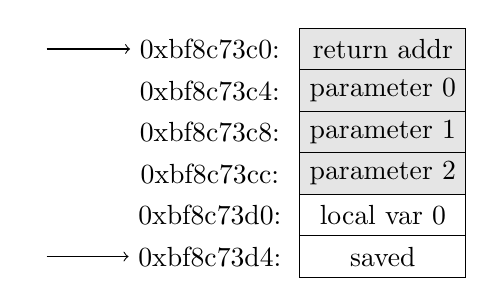
\begin{tikzpicture}
                \tikzset{x=2.5em, y=1.5em}
                \tikzstyle{mem}=[rectangle, draw, minimum width=6em, minimum height=1.5em]
                \tikzstyle{frame}=[mem, fill=black!10]

                \draw (0.0, 5.0)    node        (esp)   {\esp};
                \draw (0.0, 0.0)    node        (ebp)   {\ebp};

                \draw (2.5, 5.0)    node        (a5)    {0xbf8c73c0:};
                \draw (2.5, 4.0)    node        (a4)    {0xbf8c73c4:};
                \draw (2.5, 3.0)    node        (a3)    {0xbf8c73c8:};
                \draw (2.5, 2.0)    node        (a2)    {0xbf8c73cc:};
                \draw (2.5, 1.0)    node        (a1)    {0xbf8c73d0:};
                \draw (2.5, 0.0)    node        (a0)    {0xbf8c73d4:};

                \draw (5.0, 5.0)    node[frame] (raddr) {return addr};
                \draw (5.0, 4.0)    node[frame] (p0)    {parameter 0};
                \draw (5.0, 3.0)    node[frame] (p1)    {parameter 1};
                \draw (5.0, 2.0)    node[frame] (p2)    {parameter 2};
                \draw (5.0, 1.0)    node[mem]   (s1)    {local var 0};
                \draw (5.0, 0.0)    node[mem]   (s0)    {saved \ebp};

                \draw [->]          (esp) -- (a5);
                \draw [->]          (ebp) -- (a0);
            \end{tikzpicture}
        \end{center}
    }

    \frame{
        \frametitle{Function calls -- stack diagram}
        \begin{center}
            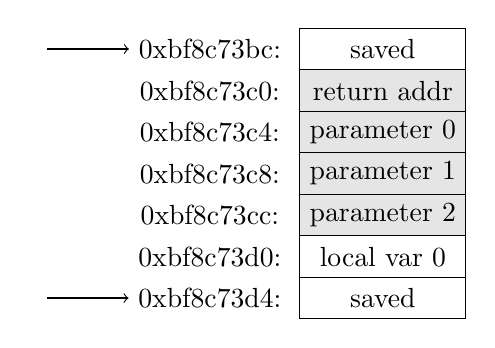
\begin{tikzpicture}
                \tikzset{x=2.5em, y=1.5em}
                \tikzstyle{mem}=[rectangle, draw, minimum width=6em, minimum height=1.5em]
                \tikzstyle{frame}=[mem, fill=black!10]

                \draw (0.0, 6.0)    node        (esp)   {\esp};
                \draw (0.0, 0.0)    node        (ebp)   {\ebp};

                \draw (2.5, 6.0)    node        (a6)    {0xbf8c73bc:};
                \draw (2.5, 5.0)    node        (a5)    {0xbf8c73c0:};
                \draw (2.5, 4.0)    node        (a4)    {0xbf8c73c4:};
                \draw (2.5, 3.0)    node        (a3)    {0xbf8c73c8:};
                \draw (2.5, 2.0)    node        (a2)    {0xbf8c73cc:};
                \draw (2.5, 1.0)    node        (a1)    {0xbf8c73d0:};
                \draw (2.5, 0.0)    node        (a0)    {0xbf8c73d4:};

                \draw (5.0, 6.0)    node[mem]   (sebp)  {saved \ebp};
                \draw (5.0, 5.0)    node[frame] (raddr) {return addr};
                \draw (5.0, 4.0)    node[frame] (p0)    {parameter 0};
                \draw (5.0, 3.0)    node[frame] (p1)    {parameter 1};
                \draw (5.0, 2.0)    node[frame] (p2)    {parameter 2};
                \draw (5.0, 1.0)    node[mem]   (s1)    {local var 0};
                \draw (5.0, 0.0)    node[mem]   (s0)    {saved \ebp};

                \draw [->]          (esp) -- (a6);
                \draw [->]          (ebp) -- (a0);
            \end{tikzpicture}
        \end{center}
    }

    \frame{
        \frametitle{Function calls -- stack diagram}
        \begin{center}
            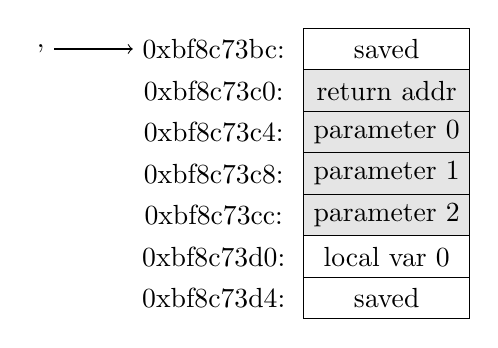
\begin{tikzpicture}
                \tikzset{x=2.5em, y=1.5em}
                \tikzstyle{mem}=[rectangle, draw, minimum width=6em, minimum height=1.5em]
                \tikzstyle{frame}=[mem, fill=black!10]

                \draw (0.0, 6.0)    node        (ep)    {\esp,\ebp};

                \draw (2.5, 6.0)    node        (a6)    {0xbf8c73bc:};
                \draw (2.5, 5.0)    node        (a5)    {0xbf8c73c0:};
                \draw (2.5, 4.0)    node        (a4)    {0xbf8c73c4:};
                \draw (2.5, 3.0)    node        (a3)    {0xbf8c73c8:};
                \draw (2.5, 2.0)    node        (a2)    {0xbf8c73cc:};
                \draw (2.5, 1.0)    node        (a1)    {0xbf8c73d0:};
                \draw (2.5, 0.0)    node        (a0)    {0xbf8c73d4:};

                \draw (5.0, 6.0)    node[mem]   (sebp)  {saved \ebp};
                \draw (5.0, 5.0)    node[frame] (raddr) {return addr};
                \draw (5.0, 4.0)    node[frame] (p0)    {parameter 0};
                \draw (5.0, 3.0)    node[frame] (p1)    {parameter 1};
                \draw (5.0, 2.0)    node[frame] (p2)    {parameter 2};
                \draw (5.0, 1.0)    node[mem]   (s1)    {local var 0};
                \draw (5.0, 0.0)    node[mem]   (s0)    {saved \ebp};

                \draw [->]          (ep) -- (a6);
            \end{tikzpicture}
        \end{center}
    }

    \frame{
        \frametitle{Function calls -- stack diagram}
        \begin{center}
            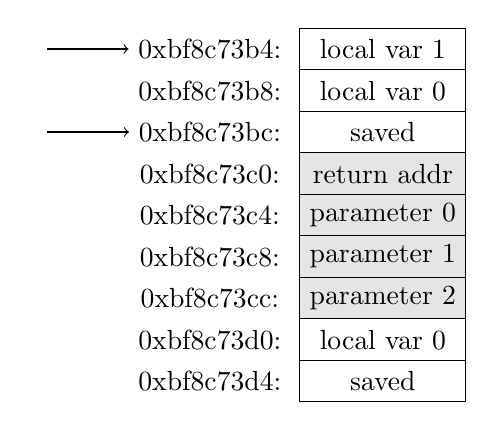
\begin{tikzpicture}
                \tikzset{x=2.5em, y=1.5em}
                \tikzstyle{mem}=[rectangle, draw, minimum width=6em, minimum height=1.5em]
                \tikzstyle{frame}=[mem, fill=black!10]

                \draw (0.0, 8.0)    node        (esp)   {\esp};
                \draw (0.0, 6.0)    node        (ebp)   {\ebp};

                \draw (2.5, 8.0)    node        (a8)    {0xbf8c73b4:};
                \draw (2.5, 7.0)    node        (a7)    {0xbf8c73b8:};
                \draw (2.5, 6.0)    node        (a6)    {0xbf8c73bc:};
                \draw (2.5, 5.0)    node        (a5)    {0xbf8c73c0:};
                \draw (2.5, 4.0)    node        (a4)    {0xbf8c73c4:};
                \draw (2.5, 3.0)    node        (a3)    {0xbf8c73c8:};
                \draw (2.5, 2.0)    node        (a2)    {0xbf8c73cc:};
                \draw (2.5, 1.0)    node        (a1)    {0xbf8c73d0:};
                \draw (2.5, 0.0)    node        (a0)    {0xbf8c73d4:};

                \draw (5.0, 8.0)    node[mem]   (v1)    {local var 1};
                \draw (5.0, 7.0)    node[mem]   (v0)    {local var 0};
                \draw (5.0, 6.0)    node[mem]   (sebp)  {saved \ebp};
                \draw (5.0, 5.0)    node[frame] (raddr) {return addr};
                \draw (5.0, 4.0)    node[frame] (p0)    {parameter 0};
                \draw (5.0, 3.0)    node[frame] (p1)    {parameter 1};
                \draw (5.0, 2.0)    node[frame] (p2)    {parameter 2};
                \draw (5.0, 1.0)    node[mem]   (s1)    {local var 0};
                \draw (5.0, 0.0)    node[mem]   (s0)    {saved \ebp};

                \draw [->]          (esp) -- (a8);
                \draw [->]          (ebp) -- (a6);
            \end{tikzpicture}
        \end{center}
    }


\subsection{Stack buffer overflow}
    \frame{
        \frametitle{Before...}
        \begin{center}
            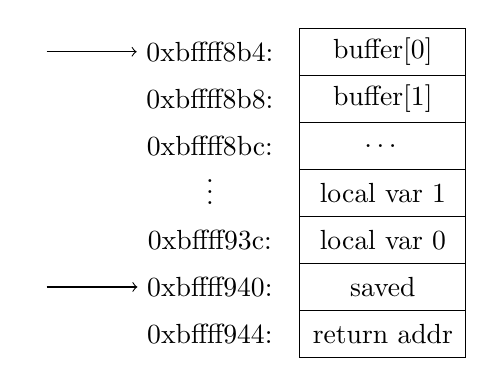
\begin{tikzpicture}
                \tikzset{x=2.5em, y=1.7em}
                \tikzstyle{mem}=[rectangle, draw, minimum width=6em, minimum height=1.7em]

                \draw (0.0, 6.0)    node        (esp)   {\esp};
                \draw (0.0, 1.0)    node        (ebp)   {\ebp};

                \draw (2.5, 6.0)    node        (a6)    {0xbffff8b4:};
                \draw (2.5, 5.0)    node        (a5)    {0xbffff8b8:};
                \draw (2.5, 4.0)    node        (a4)    {0xbffff8bc:};
                \draw (2.5, 3.2)    node        (a3)    {$\vdots$};
                \draw (2.5, 2.0)    node        (a2)    {0xbffff93c:};
                \draw (2.5, 1.0)    node        (a1)    {0xbffff940:};
                \draw (2.5, 0.0)    node        (a0)    {0xbffff944:};

                \draw (5.0, 6.0)    node[mem]   (b1)    {buffer[0]};
                \draw (5.0, 5.0)    node[mem]   (b1)    {buffer[1]};
                \draw (5.0, 4.0)    node[mem]   (b2)    {\dots};
                \draw (5.0, 3.0)    node[mem]   (v1)    {local var 1};
                \draw (5.0, 2.0)    node[mem]   (v0)    {local var 0};
                \draw (5.0, 1.0)    node[mem]   (sebp)  {saved \ebp};
                \draw (5.0, 0.0)    node[mem]   (raddr) {return addr};

                \draw [->]          (esp) -- (a6);
                \draw [->]          (ebp) -- (a1);
            \end{tikzpicture}
        \end{center}
    }

    \frame{
        \frametitle{Meanwhile...}
        \begin{center}
            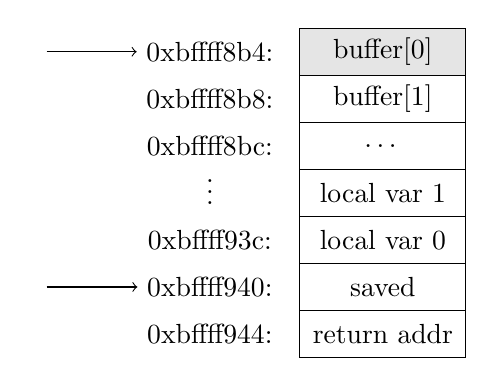
\begin{tikzpicture}
                \tikzset{x=2.5em, y=1.7em}
                \tikzstyle{mem}=[rectangle, draw, minimum width=6em, minimum height=1.7em]
                \tikzstyle{frame}=[mem, fill=black!10]

                \draw (0.0, 6.0)    node        (esp)   {\esp};
                \draw (0.0, 1.0)    node        (ebp)   {\ebp};

                \draw (2.5, 6.0)    node        (a6)    {0xbffff8b4:};
                \draw (2.5, 5.0)    node        (a5)    {0xbffff8b8:};
                \draw (2.5, 4.0)    node        (a4)    {0xbffff8bc:};
                \draw (2.5, 3.2)    node        (a3)    {$\vdots$};
                \draw (2.5, 2.0)    node        (a2)    {0xbffff93c:};
                \draw (2.5, 1.0)    node        (a1)    {0xbffff940:};
                \draw (2.5, 0.0)    node        (a0)    {0xbffff944:};

                \draw (5.0, 6.0)    node[frame] (b0)    {buffer[0]};
                \draw (5.0, 5.0)    node[mem]   (b1)    {buffer[1]};
                \draw (5.0, 4.0)    node[mem]   (b2)    {\dots};
                \draw (5.0, 3.0)    node[mem]   (v1)    {local var 1};
                \draw (5.0, 2.0)    node[mem]   (v0)    {local var 0};
                \draw (5.0, 1.0)    node[mem]   (sebp)  {saved \ebp};
                \draw (5.0, 0.0)    node[mem]   (raddr) {return addr};

                \draw [->]          (esp) -- (a6);
                \draw [->]          (ebp) -- (a1);
            \end{tikzpicture}
        \end{center}
    }

    \frame{
        \frametitle{Meanwhile...}
        \begin{center}
            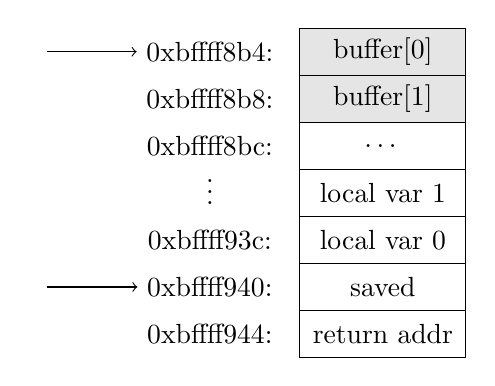
\begin{tikzpicture}
                \tikzset{x=2.5em, y=1.7em}
                \tikzstyle{mem}=[rectangle, draw, minimum width=6em, minimum height=1.7em]
                \tikzstyle{frame}=[mem, fill=black!10]

                \draw (0.0, 6.0)    node        (esp)   {\esp};
                \draw (0.0, 1.0)    node        (ebp)   {\ebp};

                \draw (2.5, 6.0)    node        (a6)    {0xbffff8b4:};
                \draw (2.5, 5.0)    node        (a5)    {0xbffff8b8:};
                \draw (2.5, 4.0)    node        (a4)    {0xbffff8bc:};
                \draw (2.5, 3.2)    node        (a3)    {$\vdots$};
                \draw (2.5, 2.0)    node        (a2)    {0xbffff93c:};
                \draw (2.5, 1.0)    node        (a1)    {0xbffff940:};
                \draw (2.5, 0.0)    node        (a0)    {0xbffff944:};

                \draw (5.0, 6.0)    node[frame] (b0)    {buffer[0]};
                \draw (5.0, 5.0)    node[frame] (b1)    {buffer[1]};
                \draw (5.0, 4.0)    node[mem]   (b2)    {\dots};
                \draw (5.0, 3.0)    node[mem]   (v1)    {local var 1};
                \draw (5.0, 2.0)    node[mem]   (v0)    {local var 0};
                \draw (5.0, 1.0)    node[mem]   (sebp)  {saved \ebp};
                \draw (5.0, 0.0)    node[mem]   (raddr) {return addr};

                \draw [->]          (esp) -- (a6);
                \draw [->]          (ebp) -- (a1);
            \end{tikzpicture}
        \end{center}
    }

    \frame{
        \frametitle{Meanwhile...}
        \begin{center}
            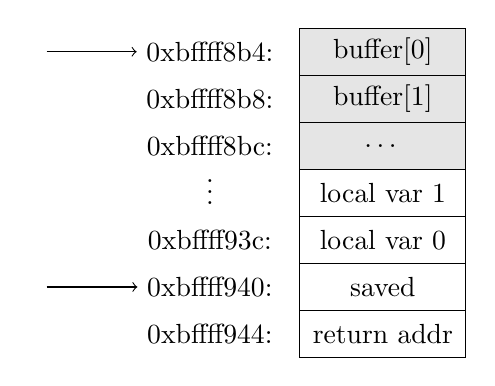
\begin{tikzpicture}
                \tikzset{x=2.5em, y=1.7em}
                \tikzstyle{mem}=[rectangle, draw, minimum width=6em, minimum height=1.7em]
                \tikzstyle{frame}=[mem, fill=black!10]

                \draw (0.0, 6.0)    node        (esp)   {\esp};
                \draw (0.0, 1.0)    node        (ebp)   {\ebp};

                \draw (2.5, 6.0)    node        (a6)    {0xbffff8b4:};
                \draw (2.5, 5.0)    node        (a5)    {0xbffff8b8:};
                \draw (2.5, 4.0)    node        (a4)    {0xbffff8bc:};
                \draw (2.5, 3.2)    node        (a3)    {$\vdots$};
                \draw (2.5, 2.0)    node        (a2)    {0xbffff93c:};
                \draw (2.5, 1.0)    node        (a1)    {0xbffff940:};
                \draw (2.5, 0.0)    node        (a0)    {0xbffff944:};

                \draw (5.0, 6.0)    node[frame] (b0)    {buffer[0]};
                \draw (5.0, 5.0)    node[frame] (b1)    {buffer[1]};
                \draw (5.0, 4.0)    node[frame] (b2)    {\dots};
                \draw (5.0, 3.0)    node[mem]   (v1)    {local var 1};
                \draw (5.0, 2.0)    node[mem]   (v0)    {local var 0};
                \draw (5.0, 1.0)    node[mem]   (sebp)  {saved \ebp};
                \draw (5.0, 0.0)    node[mem]   (raddr) {return addr};

                \draw [->]          (esp) -- (a6);
                \draw [->]          (ebp) -- (a1);
            \end{tikzpicture}
        \end{center}
    }

    \frame{
        \frametitle{Meanwhile...}
        \begin{center}
            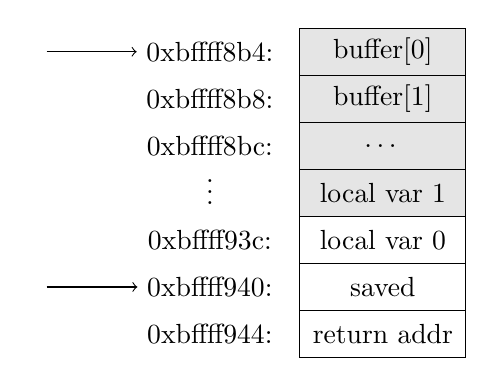
\begin{tikzpicture}
                \tikzset{x=2.5em, y=1.7em}
                \tikzstyle{mem}=[rectangle, draw, minimum width=6em, minimum height=1.7em]
                \tikzstyle{frame}=[mem, fill=black!10]

                \draw (0.0, 6.0)    node        (esp)   {\esp};
                \draw (0.0, 1.0)    node        (ebp)   {\ebp};

                \draw (2.5, 6.0)    node        (a6)    {0xbffff8b4:};
                \draw (2.5, 5.0)    node        (a5)    {0xbffff8b8:};
                \draw (2.5, 4.0)    node        (a4)    {0xbffff8bc:};
                \draw (2.5, 3.2)    node        (a3)    {$\vdots$};
                \draw (2.5, 2.0)    node        (a2)    {0xbffff93c:};
                \draw (2.5, 1.0)    node        (a1)    {0xbffff940:};
                \draw (2.5, 0.0)    node        (a0)    {0xbffff944:};

                \draw (5.0, 6.0)    node[frame] (b0)    {buffer[0]};
                \draw (5.0, 5.0)    node[frame] (b1)    {buffer[1]};
                \draw (5.0, 4.0)    node[frame] (b2)    {\dots};
                \draw (5.0, 3.0)    node[frame] (v1)    {local var 1};
                \draw (5.0, 2.0)    node[mem]   (v0)    {local var 0};
                \draw (5.0, 1.0)    node[mem]   (sebp)  {saved \ebp};
                \draw (5.0, 0.0)    node[mem]   (raddr) {return addr};

                \draw [->]          (esp) -- (a6);
                \draw [->]          (ebp) -- (a1);
            \end{tikzpicture}
        \end{center}
    }

    \frame{
        \frametitle{Boom!}
        \begin{center}
            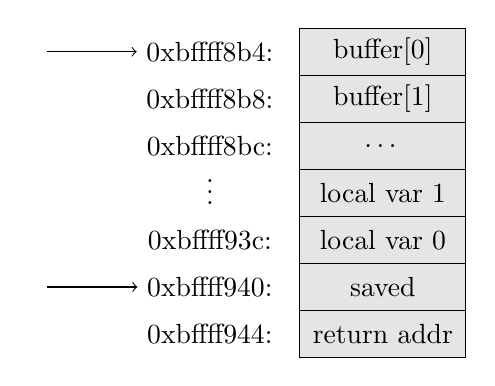
\begin{tikzpicture}
                \tikzset{x=2.5em, y=1.7em}
                \tikzstyle{mem}=[rectangle, draw, minimum width=6em, minimum height=1.7em]
                \tikzstyle{frame}=[mem, fill=black!10]

                \draw (0.0, 6.0)    node        (esp)   {\esp};
                \draw (0.0, 1.0)    node        (ebp)   {\ebp};

                \draw (2.5, 6.0)    node        (a6)    {0xbffff8b4:};
                \draw (2.5, 5.0)    node        (a5)    {0xbffff8b8:};
                \draw (2.5, 4.0)    node        (a4)    {0xbffff8bc:};
                \draw (2.5, 3.2)    node        (a3)    {$\vdots$};
                \draw (2.5, 2.0)    node        (a2)    {0xbffff93c:};
                \draw (2.5, 1.0)    node        (a1)    {0xbffff940:};
                \draw (2.5, 0.0)    node        (a0)    {0xbffff944:};

                \draw (5.0, 6.0)    node[frame] (b0)    {buffer[0]};
                \draw (5.0, 5.0)    node[frame] (b1)    {buffer[1]};
                \draw (5.0, 4.0)    node[frame] (b2)    {\dots};
                \draw (5.0, 3.0)    node[frame] (v1)    {local var 1};
                \draw (5.0, 2.0)    node[frame] (v0)    {local var 0};
                \draw (5.0, 1.0)    node[frame] (sebp)  {saved \ebp};
                \draw (5.0, 0.0)    node[frame] (raddr) {return addr};

                \draw [->]          (esp) -- (a6);
                \draw [->]          (ebp) -- (a1);
            \end{tikzpicture}
        \end{center}
    }



\subsection{Gadgets}
    \frame{
        \frametitle{What is a gadget?}
        \begin{itemize}
            \item attacker searches for short instruction sequences that perform small tasks and end with \ret \\
                  \lto\ for example \pop ing some values into registers
            \item gadget: combination of one or more addresses of short instruction sequences and the values that they should \pop\ off the stack
            \item \payload: chain of gadgets
        \end{itemize}
    }

    \frame{
        \frametitle{A very simple gadget}
        \begin{center}
            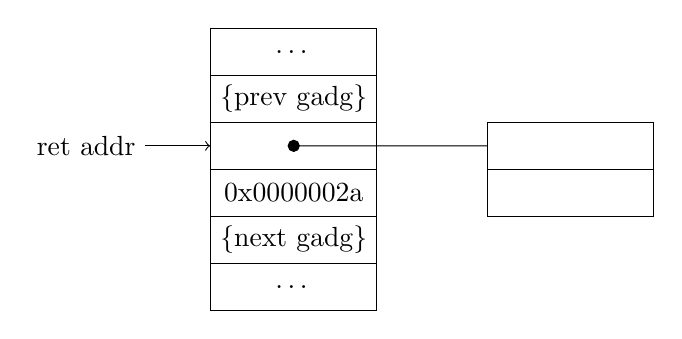
\begin{tikzpicture}
                \tikzset{x=2.5em, y=1.7em, radius=2pt, fill=black}
                \tikzstyle{mem}=[rectangle, draw, minimum width=6em, minimum height=1.7em]

                % annotations
                \draw (0.0, 3.0)    node        (ret)   {ret addr};

                % stack
                \draw (3.0, 5.0)    node[mem]   (s5)    {\dots};
                \draw (3.0, 4.0)    node[mem]   (s4)    {\{prev gadg\}};
                \draw (3.0, 3.0)    node[mem]   (s3)    {};
                \draw (3.0, 2.0)    node[mem]   (s2)    {0x0000002a};
                \draw (3.0, 1.0)    node[mem]   (s1)    {\{next gadg\}};
                \draw (3.0, 0.0)    node[mem]   (s0)    {\dots};

                % first fake stack frame
                \draw (7.0, 3.0)    node[mem]   (i0)    {\pop\ \eax};
                \draw (7.0, 2.0)    node[mem]   (i1)    {\ret};

                % annotation arrows
                \draw [->]          (ret) -- (s3);

                % memory pointer arrows
                \filldraw           (s3.center)  circle -- (i0.west);
            \end{tikzpicture}
        \end{center}
    }
